\chapter{Experimento}
Este capítulo descreve o experimento visando avaliar a eficácia, em termos de precision, recall e f-measure \cite{goutte2005probabilistic} a proposta. Dessa forma,  o experimento compara a proposta com RiMOM-2015 e LogMap. Vale a pena ressaltar que a ferramenta Lily não pôde ser avaliada por inviabilização do acesso à solução.

O capítulo está dividido em três seções: planejamento, execução e análise dos dados. 

\section*{Planejamento do experimento}

Nesta seção, será detalhado o planejamento do experimento que foi projetado para este trabalho. Destro do planejamento, encontra-se a definição da questão de pesquisa e derivação de hipóteses, a seleção das variáveis dependentes e independentes a identificação da unidade experimental e a seleção do modelo experimental que será utilizado.

O experimento adotado é do tipo comparativo, no qual será comparada a ferramenta proposta com as ferramentas RiMOM-2015 e LogMap. O contexto do experimento é acadêmico, posto que executado em um laboratório, mas executando algoritmos com dados reais. Nas próximas subseções, o planejamento do experimento será descrito.

\subsection*{Hipóteses de pesquisa}

Como mencionado no início deste capítulo, este experimento visa avaliar a proposta com relação às métricas precision, recall e f-measure. Levando em consideração as questões de pesquisa a seguir:

\textbf{Q1} Existem diferença na eficácia entre RiMOM-2015, LogMap e a solução proposta? Se sim, qual abordagem foi melhor?
A questão de pesquisa acima implica nas seguintes hipóteses de pesquisa:

\begin{itemize}
\item H1-0: A métrica precision entre apresentada pelas abordagens é igual.
\item H1-1: A métrica precision entre apresentada pelas abordagens é diferente.
\item H2-0: A métrica recall entre apresentada pelas abordagens é igual.
\item H2-1: A métrica recall entre apresentada pelas abordagens é diferente.
\item H3-0: A métrica f-measure entre apresentada pelas abordagens é igual.
\item H3-1: A métrica f-measure entre apresentada pelas abordagens é diferente.
\end{itemize}

Caso a hipótese nula seja refutada (indicando diferença), uma análise das métricas será executada para que se possa concluir qual ferramenta se saiu melhor.
A tabela \ref{tab:hypothesis} define formalmente as hipóteses de pesquisa supracitadas. P, R e F são funções que retornam, respectivamente o precision, o recall e f-measure, com relação às abordagens F1 (RiMOM-2015), F2 (LogMap) e F3 (Proposta).

\begin{table}[h]
\centering
\caption{Formalização das hipóteses}
\label{tab:hypothesis}
\begin{tabular}{|c|c|c|}
\hline
Hipótese & Hipótese Nula & Hipótese Alternativa \\ \hline
H1       & H1-0:$ P(F1) = P(F2) = P(F3) $ & H1-1:$ P(F1) \not= P(F2) \not= P(F3) $                    \\ \hline
H2       & H2-0:$ R(F1) = R(F2) = R(F3) $ & H2-1:$ R(F1) \not= R(F2) \not= R(F3) $                    \\ \hline
H3       & H3-0:$ F(F1) = F(F2) = F(F3) $ & H3-1:$ F(F1) \not= F(F2) \not= F(F3) $                    \\ \hline
\end{tabular}
\end{table}

\subsection*{Seleção de Variáveis}
Seguindo o planejamento, é necessário definir as variáveis contidas no experimento. Primeiro, as variáveis independentes, também chamadas de fatores, serão apresentadas. Logo em seguida, as variáveis dependentes, no caso as métricas, serão detalhadas.

As variáveis independentes são as seguintes:
\begin{itemize}
\item \textbf{Ferramenta} : Esta variável especifica qual a ferramenta de alinhamento será avaliada
\end{itemize}

Os níveis de fatores apresentados acima serão definidos na tabela \ref{tab:factor_levels}. As variáveis dependentes (métricas) são definidas abaixo:

\begin{itemize}
\item \textbf{Precision} (P): Esta variável representa a precisão para cada um dos níveis avaliados. A definição formal para esta métrica é descrita pela equação abaixo:

\begin{equation}
P = \dfrac{|{A}\cap{B}|}{|A|}
\end{equation}

\item \textbf{Recall} (R): Esta variável representa o recall para cada um dos níveis avaliados. A definição formal para esta métrica é descrita pela equação abaixo:

\begin{equation}
R = \dfrac{|{A}\cap{B}|}{|B|}
\end{equation}

\item \textbf{F-measure} (F): Esta variável representa o f-measure para cada um dos níveis avaliados. A definição formal para esta métrica é descrita pela equação abaixo:

\begin{equation}
F = \dfrac{{2}\cdot{P}\cdot{R}}{P+R}
\end{equation}

\end{itemize}

\begin{table}[]
\centering
\caption{Níveis de fatores}
\label{tab:factor_levels}
\begin{tabular}{|c|c|c|}
\hline
\textbf{Fator}              & \textbf{Nível} & \textbf{Descrição}    \\ \hline
\multirow{3}{*}{Ferramenta} & F1             & Ferramenta RiMOM-2015 \\ \cline{2-3} 
                            & F2             & Ferramenta LogMap     \\ \cline{2-3} 
                            & F3             & Proprosta             \\ \hline
\end{tabular}
\end{table}

\subsection*{Unidades de Experimento}
A unidade experimental deste estudo é composto por três datasets (DBPedia\footnote{http://www.dbpedia.pt}, IBGE\footnote{http://cidades.ibge.gov.br
}, Alagoas em Dados\footnote{http://dados.al.gov.br/dataset}), que contêm as cidades do estado de Alagoas. Os datasets  foram extraídos e transformados em RDF  seguindo a especificação da ontologia do dbpedia\footnote{http://dbpedia.org/ontology/}, que podem ser conferidos através do link \url{https://goo.gl/TkzStn}.

Através da composição entre os elementos da unidade experimental (datasets), montamos o cenário de avaliação das ferramentas. A tabela \ref{tab:cenarios} apresenta os cenários. Vale a pensa ressaltar que não há a necessidade de cenários em que um dataset é alinhado com ele mesmo, pois não há recursos duplicados nos datasets. Além disso, não há a necessidade de criar cenário em que haja a permutação entre os datasets.

\begin{table}[h]
\centering
\caption{Cenários de alinhamento}
\label{tab:cenarios}
\begin{tabular}{|c|c|}
\hline
\textbf{Cenário} & \textbf{Datasets}          \\ \hline
C1               & DBPedia X IBGE             \\ \hline
C2               & DBPedia X Alagoas em Dados \\ \hline
C3               & IBGE X Alagoas em Dados    \\ \hline
\end{tabular}
\end{table}

Para este experimento, com exceção dos dados fornecidos pela dbpedia, os demais foram transformados para RDF através da ferramenta OpenRefine e persistidos no Virtuoso.  
Todo o experimento foi executado utilizando a entidade City como conceito principal. A escolha desse conceito se deve ao fato deste ser o principal conceito.

\subsection*{Seleção do Projeto Experimental}
Levando em consideração as diversas classificações de experimento \cite{montgomery2012design}, o presente experimento é classificado como fatorial completo com blocagem. A blocagem foi escolhida com o objetivo de suprimir os efeitos dos datasets nas variáveis resposta. Para cada cenário houve a execução de todos os fatores, garantindo a completude do experimento. Dessa forma temos 3 cenários possíveis, com 3 execuções em cada um deles, totalizando 9 execuções.

\section*{Execução do experimento}
Esta seção descreve a execução do experimento que foi planejado na seção anterior, ou seja, descreve quais instrumentos foram utilizados, bem como a narrativa de execução do experimento.

\subsection*{Preparação e instrumentação}
Inicialmente é necessário preparar o ambiente em que os alinhamentos serão executados. As ferramentas utilizadas, bem como suas versões são descritas a seguir:

\begin{itemize}
\item Virtuoso RDF Store - 07.20.3217;
\item Python - 2.7;
\item OpenJDK 64-Bit Server VM (build 25.111-b14, mixed mode)

\end{itemize}

Para isolar os efeitos entre as execuções, todo o experimento foi conduzido em um container do Docker, que permitem isolar as aplicações, fazendo com que as aplicações sejam executadas em ambientes idênticos.

\subsection*{Narrativa do experimento}
A Figura \ref{fig:experiment} apresenta os passos de execução de cada alinhamento, que são descritos abaixo:
\begin{itemize}
\item Construir container com as configurações zeradas;
\item Carregar dos dados;
\item Executar ferramenta dentro do container;
\item Coletar dados de alinhamento;
\item Destruir container;
\item Analisar dados;
\end{itemize}

\begin{figure}[h]
	\centering
	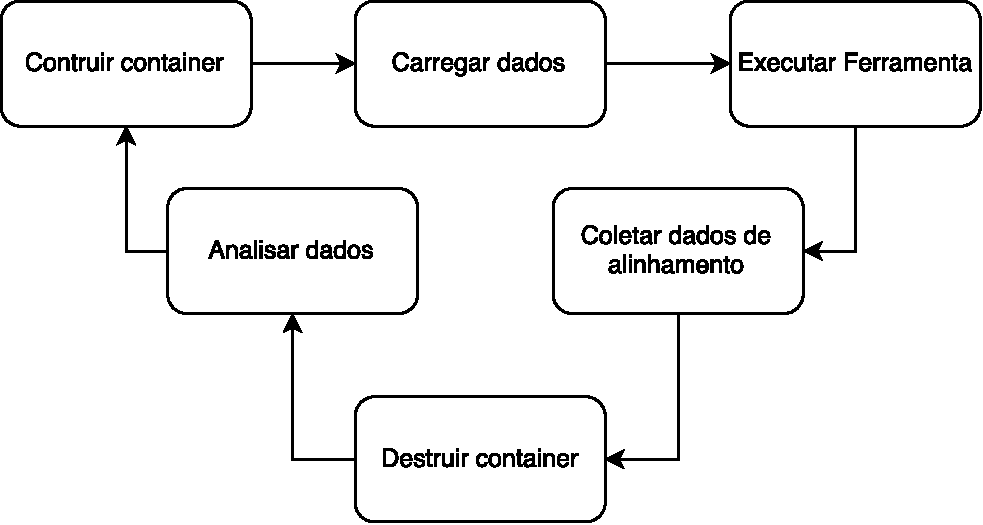
\includegraphics[width=0.9\textwidth]{./imagens/experimento.pdf}
    \caption{Processo de execução do experimento}
	\label{fig:experiment}
\end{figure}

\subsection*{Análise de Ameaças à Validade}
Embora todo experimento tenha sido projetado para minimizar possíveis ameaças que comprometam suas conclusões, existem algumas ameaças que devem ser mencionadas. Uma possível ameaça à validade do experimento é com relação a quantidade de amostras, o número de recursos, bem como a quantidade de datasets pode influenciar o resultado do alinhamento.
Levando isso em consideração, na próxima seção, os dados obtidos a partir da execução do experimento serão analisados.

\subsection*{Análise dos dados}
O experimento foi conduzido de acordo com o planejamento descrito anteriormente neste capítulo, depois da execução, os datasets de alinhamento eram coletados. Os dados de precision, recall e f-measure eram calculados através de script Python de acordo com as funções especificadas anteriormente.
Ao longo desta seção, uma análise descritiva dos dados obtidos será conduzida, esta análise envolve a apresentação das métricas referentes a cada cenário. Vale a pensa ressaltar que as ferramentas RiMOM-2015 e LogMap não foram capazes de alinhar instâncias dos datasets, recebendo 0 (zero) nas métricas precision e recall. Podemos levantar alguns motivos para o baixo desempenho das ferramentas apresentadas, porém não é possível afirmar com certeza, pois em nenhum dos artigos foi apresentada as alterações que essas soluções sofreram para suportar o alinhamento de dados.

Os alinhamentos gerados para cada um dos cenários podem ser acessados através do link \url{https://goo.gl/RbIuBH}. Dessa forma, as figuras \ref{fig:cenario1}, \ref{fig:cenario2} e \ref{fig:cenario3} apresentam as métricas de precision, recall e f-measure da proposta nos cenários C1, C2 e C3 respectivamente. 
\begin{center}
\begin{figure}
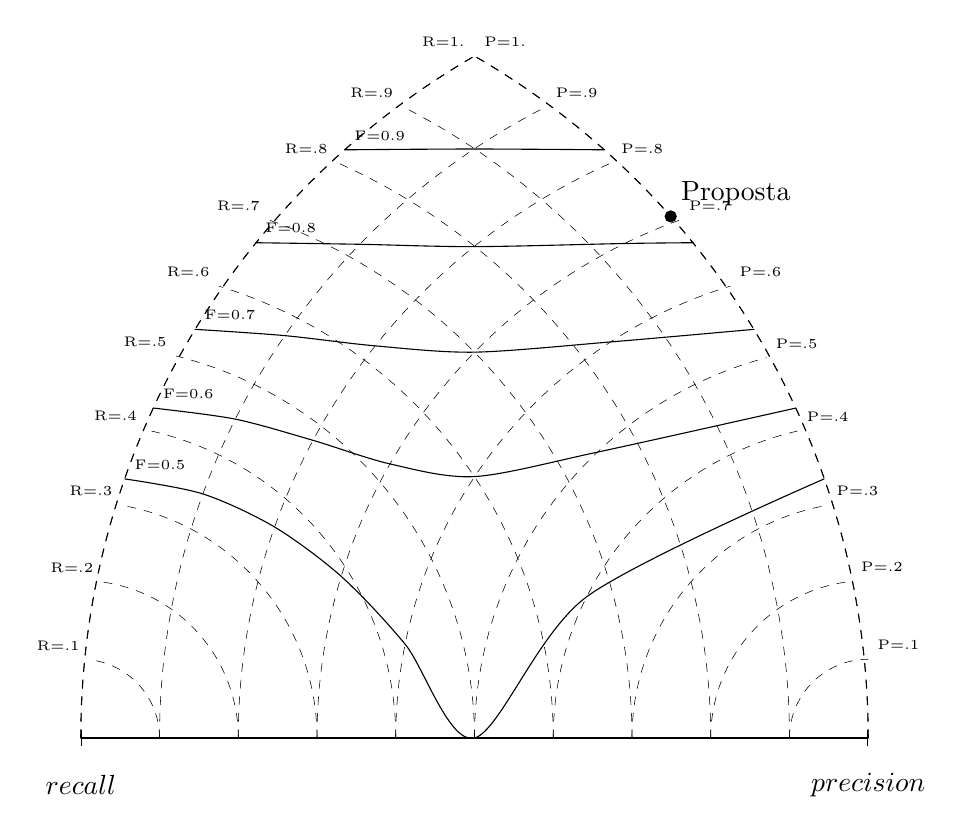
\begin{tikzpicture}[cap=round]{H}
%\draw[step=1cm,very thin,color=gray] (0,0) grid (10.0,9.0);
\draw[|-|] (-0,0) -- (10,0);
\draw[dashed,very thin] (10,0) arc (0:60:10cm);
\draw[dashed,very thin] (0,0) arc (180:120:10cm);
\draw[dashed] (10,0) arc (0:60:10cm) node[anchor=south east]  {{\tiny R=1.}};
\draw[dashed,very thin] (9,0) arc (0:63:9cm) node[anchor=south east] {{\tiny R=.9}};
\draw[dashed,very thin] (8,0) arc (0:66:8cm) node[anchor=south east]  {{\tiny R=.8}};
\draw[dashed,very thin] (7,0) arc (0:70:7cm) node[anchor=south east]  {{\tiny R=.7}};
\draw[dashed,very thin] (6,0) arc (0:73:6cm) node[anchor=south east]  {{\tiny R=.6}};
\draw[dashed,very thin] (5,0) arc (0:76:5cm) node[anchor=south east] {{\tiny R=.5}};
\draw[dashed,very thin] (4,0) arc (0:78:4cm) node[anchor=south east] {{\tiny R=.4}};
\draw[dashed,very thin] (3,0) arc (0:80:3cm) node[anchor=south east] {{\tiny R=.3}};
\draw[dashed,very thin] (2,0) arc (0:82:2cm) node[anchor=south east] {{\tiny R=.2}};
\draw[dashed,very thin] (1,0) arc (0:84:1cm) node[anchor=south east] {{\tiny R=.1}};
\draw[dashed] (0,0) arc (180:120:10cm) node[anchor=south west] {{\tiny P=1.}};
\draw[dashed,very thin] (1,0) arc (180:117:9cm) node[anchor=south west] {{\tiny P=.9}};
\draw[dashed,very thin] (2,0) arc (180:114:8cm) node[anchor=south west] {{\tiny P=.8}};
\draw[dashed,very thin] (3,0) arc (180:110:7cm) node[anchor=south west] {{\tiny P=.7}};
\draw[dashed,very thin] (4,0) arc (180:107:6cm) node[anchor=south west] {{\tiny P=.6}};
\draw[dashed,very thin] (5,0) arc (180:105:5cm) node[anchor=south west] {{\tiny P=.5}};
\draw[dashed,very thin] (6,0) arc (180:103:4cm) node[anchor=south west] {{\tiny P=.4}};
\draw[dashed,very thin] (7,0) arc (180:100:3cm) node[anchor=south west] {{\tiny P=.3}};
\draw[dashed,very thin] (8,0) arc (180:96:2cm) node[anchor=south west] {{\tiny P=.2}};
\draw[dashed,very thin] (9,0) arc (180:90:1cm) node[anchor=south west] {{\tiny P=.1}};
\draw (0.56,3.29) node[anchor=south west] {\tiny{F=0.5}};
\draw plot[smooth] coordinates { (0.56,3.29) (1.55,3.10) (2.46,2.68) (3.31,2.05) (4.12,1.19) (5.00,0.00) (6.42,1.79) (9.44,3.29)};
\draw (0.92,4.19) node[anchor=south west] {\tiny{F=0.6}};
\draw plot[smooth] coordinates { (0.92,4.19) (1.96,4.05) (2.95,3.78) (3.93,3.48) (5.00,3.32) (6.56,3.63) (9.08,4.19)};
\draw (1.45,5.19) node[anchor=south west] {\tiny{F=0.7}};
\draw plot[smooth] coordinates { (1.45,5.19) (2.59,5.11) (3.74,4.98) (5.00,4.90) (6.73,5.03) (8.55,5.19)};
\draw (2.22,6.29) node[anchor=south west] {\tiny{F=0.8}};
\draw plot[smooth] coordinates { (2.22,6.29) (3.54,6.27) (5.00,6.24) (6.91,6.28) (7.78,6.29)};
\draw (3.35,7.47) node[anchor=south west] {\tiny{F=0.9}};
\draw plot[smooth] coordinates { (3.35,7.47) (5.00,7.48) (6.65,7.47)};
\draw (0,-0.6) node {$recall$};
\draw (10,-0.6) node {$precision$};
%\draw (-0.2,0) node {0}; 
%\draw (10.2,0) node {1}; 
\draw plot[mark=*,] coordinates {(7.49155555,6.62394108075)};
\draw (7.50155555,6.63394108075) node[anchor=south west] {Proposta};
\end{tikzpicture}
\caption{Métricas de precision, recall e f-measure no cenário 1}
\label{fig:cenario1}
\end{figure}

\begin{figure}
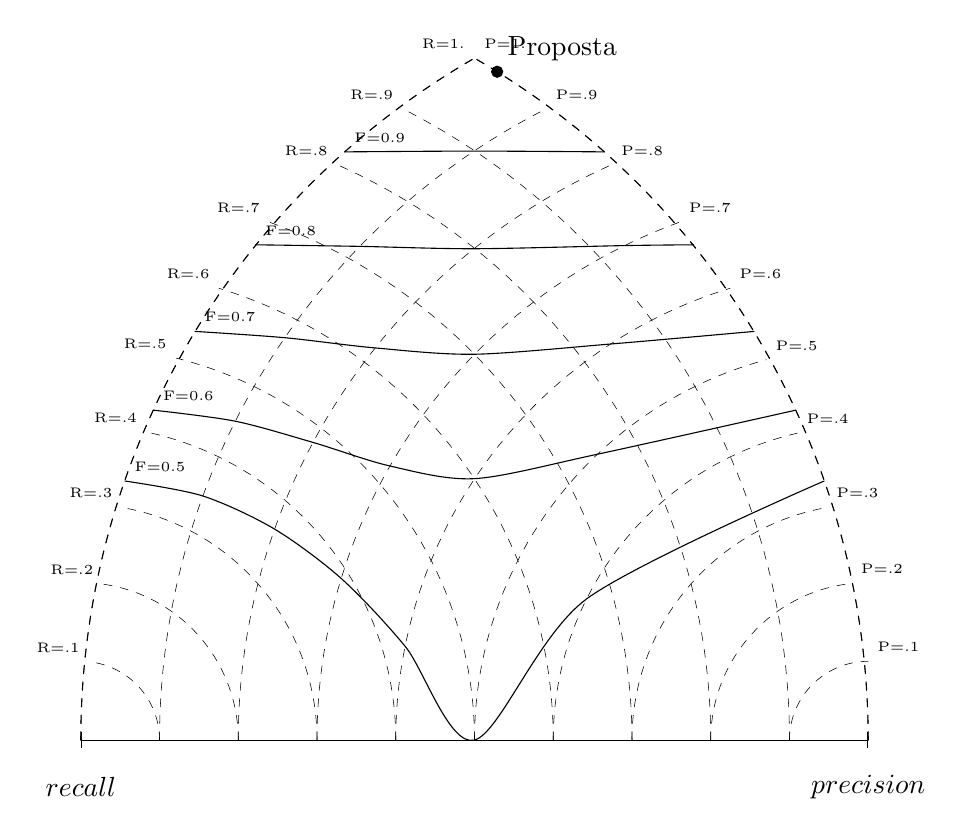
\begin{tikzpicture}[cap=round]{H}
%\draw[step=1cm,very thin,color=gray] (0,0) grid (10.0,9.0);
\draw[|-|] (-0,0) -- (10,0);
\draw[dashed,very thin] (10,0) arc (0:60:10cm);
\draw[dashed,very thin] (0,0) arc (180:120:10cm);
\draw[dashed] (10,0) arc (0:60:10cm) node[anchor=south east]  {{\tiny R=1.}};
\draw[dashed,very thin] (9,0) arc (0:63:9cm) node[anchor=south east] {{\tiny R=.9}};
\draw[dashed,very thin] (8,0) arc (0:66:8cm) node[anchor=south east]  {{\tiny R=.8}};
\draw[dashed,very thin] (7,0) arc (0:70:7cm) node[anchor=south east]  {{\tiny R=.7}};
\draw[dashed,very thin] (6,0) arc (0:73:6cm) node[anchor=south east]  {{\tiny R=.6}};
\draw[dashed,very thin] (5,0) arc (0:76:5cm) node[anchor=south east] {{\tiny R=.5}};
\draw[dashed,very thin] (4,0) arc (0:78:4cm) node[anchor=south east] {{\tiny R=.4}};
\draw[dashed,very thin] (3,0) arc (0:80:3cm) node[anchor=south east] {{\tiny R=.3}};
\draw[dashed,very thin] (2,0) arc (0:82:2cm) node[anchor=south east] {{\tiny R=.2}};
\draw[dashed,very thin] (1,0) arc (0:84:1cm) node[anchor=south east] {{\tiny R=.1}};
\draw[dashed] (0,0) arc (180:120:10cm) node[anchor=south west] {{\tiny P=1.}};
\draw[dashed,very thin] (1,0) arc (180:117:9cm) node[anchor=south west] {{\tiny P=.9}};
\draw[dashed,very thin] (2,0) arc (180:114:8cm) node[anchor=south west] {{\tiny P=.8}};
\draw[dashed,very thin] (3,0) arc (180:110:7cm) node[anchor=south west] {{\tiny P=.7}};
\draw[dashed,very thin] (4,0) arc (180:107:6cm) node[anchor=south west] {{\tiny P=.6}};
\draw[dashed,very thin] (5,0) arc (180:105:5cm) node[anchor=south west] {{\tiny P=.5}};
\draw[dashed,very thin] (6,0) arc (180:103:4cm) node[anchor=south west] {{\tiny P=.4}};
\draw[dashed,very thin] (7,0) arc (180:100:3cm) node[anchor=south west] {{\tiny P=.3}};
\draw[dashed,very thin] (8,0) arc (180:96:2cm) node[anchor=south west] {{\tiny P=.2}};
\draw[dashed,very thin] (9,0) arc (180:90:1cm) node[anchor=south west] {{\tiny P=.1}};
\draw (0.56,3.29) node[anchor=south west] {\tiny{F=0.5}};
\draw plot[smooth] coordinates { (0.56,3.29) (1.55,3.10) (2.46,2.68) (3.31,2.05) (4.12,1.19) (5.00,0.00) (6.42,1.79) (9.44,3.29)};
\draw (0.92,4.19) node[anchor=south west] {\tiny{F=0.6}};
\draw plot[smooth] coordinates { (0.92,4.19) (1.96,4.05) (2.95,3.78) (3.93,3.48) (5.00,3.32) (6.56,3.63) (9.08,4.19)};
\draw (1.45,5.19) node[anchor=south west] {\tiny{F=0.7}};
\draw plot[smooth] coordinates { (1.45,5.19) (2.59,5.11) (3.74,4.98) (5.00,4.90) (6.73,5.03) (8.55,5.19)};
\draw (2.22,6.29) node[anchor=south west] {\tiny{F=0.8}};
\draw plot[smooth] coordinates { (2.22,6.29) (3.54,6.27) (5.00,6.24) (6.91,6.28) (7.78,6.29)};
\draw (3.35,7.47) node[anchor=south west] {\tiny{F=0.9}};
\draw plot[smooth] coordinates { (3.35,7.47) (5.00,7.48) (6.65,7.47)};
\draw (0,-0.6) node {$recall$};
\draw (10,-0.6) node {$precision$};
%\draw (-0.2,0) node {0}; 
%\draw (10.2,0) node {1}; 
\draw plot[mark=*,] coordinates {(5.2877368,8.48762861664)};
\draw (5.2977368,8.49762861664) node[anchor=south west] {Proposta};
\end{tikzpicture}
\caption{Métricas de precision, recall e f-measure no cenário 2}
\label{fig:cenario2}
\end{figure}

\begin{figure}
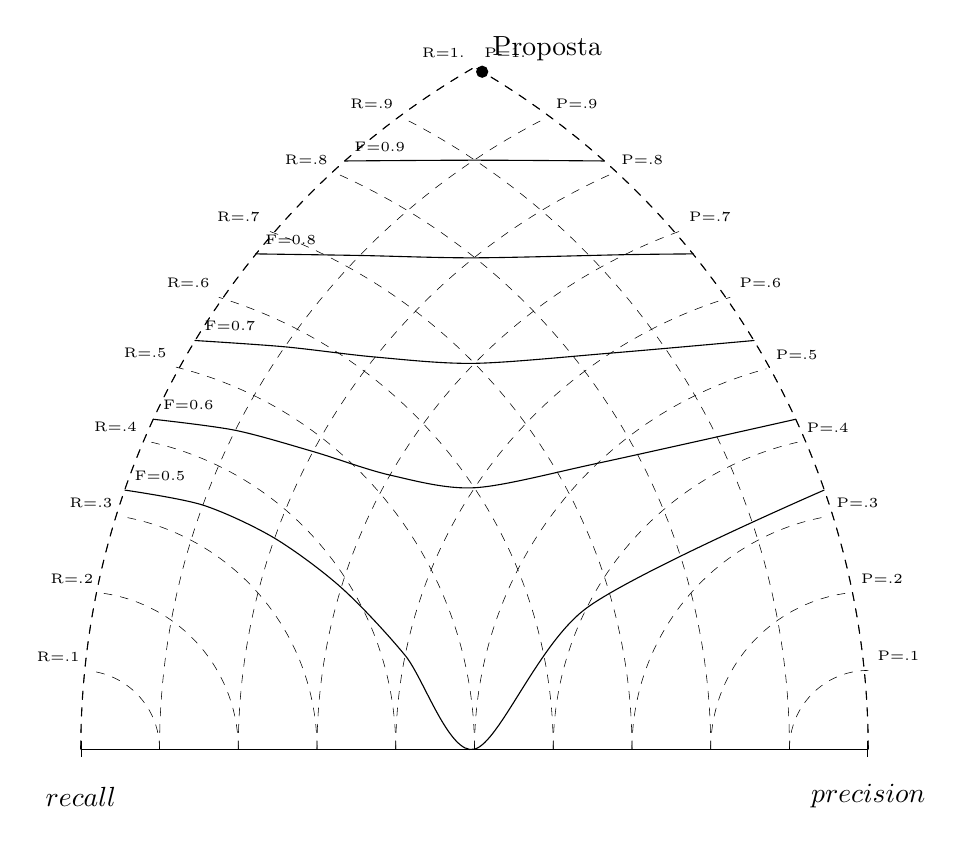
\begin{tikzpicture}[cap=round]{H}
%\draw[step=1cm,very thin,color=gray] (0,0) grid (10.0,9.0);
\draw[|-|] (-0,0) -- (10,0);
\draw[dashed,very thin] (10,0) arc (0:60:10cm);
\draw[dashed,very thin] (0,0) arc (180:120:10cm);
\draw[dashed] (10,0) arc (0:60:10cm) node[anchor=south east]  {{\tiny R=1.}};
\draw[dashed,very thin] (9,0) arc (0:63:9cm) node[anchor=south east] {{\tiny R=.9}};
\draw[dashed,very thin] (8,0) arc (0:66:8cm) node[anchor=south east]  {{\tiny R=.8}};
\draw[dashed,very thin] (7,0) arc (0:70:7cm) node[anchor=south east]  {{\tiny R=.7}};
\draw[dashed,very thin] (6,0) arc (0:73:6cm) node[anchor=south east]  {{\tiny R=.6}};
\draw[dashed,very thin] (5,0) arc (0:76:5cm) node[anchor=south east] {{\tiny R=.5}};
\draw[dashed,very thin] (4,0) arc (0:78:4cm) node[anchor=south east] {{\tiny R=.4}};
\draw[dashed,very thin] (3,0) arc (0:80:3cm) node[anchor=south east] {{\tiny R=.3}};
\draw[dashed,very thin] (2,0) arc (0:82:2cm) node[anchor=south east] {{\tiny R=.2}};
\draw[dashed,very thin] (1,0) arc (0:84:1cm) node[anchor=south east] {{\tiny R=.1}};
\draw[dashed] (0,0) arc (180:120:10cm) node[anchor=south west] {{\tiny P=1.}};
\draw[dashed,very thin] (1,0) arc (180:117:9cm) node[anchor=south west] {{\tiny P=.9}};
\draw[dashed,very thin] (2,0) arc (180:114:8cm) node[anchor=south west] {{\tiny P=.8}};
\draw[dashed,very thin] (3,0) arc (180:110:7cm) node[anchor=south west] {{\tiny P=.7}};
\draw[dashed,very thin] (4,0) arc (180:107:6cm) node[anchor=south west] {{\tiny P=.6}};
\draw[dashed,very thin] (5,0) arc (180:105:5cm) node[anchor=south west] {{\tiny P=.5}};
\draw[dashed,very thin] (6,0) arc (180:103:4cm) node[anchor=south west] {{\tiny P=.4}};
\draw[dashed,very thin] (7,0) arc (180:100:3cm) node[anchor=south west] {{\tiny P=.3}};
\draw[dashed,very thin] (8,0) arc (180:96:2cm) node[anchor=south west] {{\tiny P=.2}};
\draw[dashed,very thin] (9,0) arc (180:90:1cm) node[anchor=south west] {{\tiny P=.1}};
\draw (0.56,3.29) node[anchor=south west] {\tiny{F=0.5}};
\draw plot[smooth] coordinates { (0.56,3.29) (1.55,3.10) (2.46,2.68) (3.31,2.05) (4.12,1.19) (5.00,0.00) (6.42,1.79) (9.44,3.29)};
\draw (0.92,4.19) node[anchor=south west] {\tiny{F=0.6}};
\draw plot[smooth] coordinates { (0.92,4.19) (1.96,4.05) (2.95,3.78) (3.93,3.48) (5.00,3.32) (6.56,3.63) (9.08,4.19)};
\draw (1.45,5.19) node[anchor=south west] {\tiny{F=0.7}};
\draw plot[smooth] coordinates { (1.45,5.19) (2.59,5.11) (3.74,4.98) (5.00,4.90) (6.73,5.03) (8.55,5.19)};
\draw (2.22,6.29) node[anchor=south west] {\tiny{F=0.8}};
\draw plot[smooth] coordinates { (2.22,6.29) (3.54,6.27) (5.00,6.24) (6.91,6.28) (7.78,6.29)};
\draw (3.35,7.47) node[anchor=south west] {\tiny{F=0.9}};
\draw plot[smooth] coordinates { (3.35,7.47) (5.00,7.48) (6.65,7.47)};
\draw (0,-0.6) node {$recall$};
\draw (10,-0.6) node {$precision$};
%\draw (-0.2,0) node {0}; 
%\draw (10.2,0) node {1}; 
\draw plot[mark=*,] coordinates {(5.0975198,8.6032140441)};
\draw (5.1075198,8.6132140441) node[anchor=south west] {Proposta};
\end{tikzpicture}
\caption{Métricas de precision, recall e f-measure no cenário 3}
\label{fig:cenario3}
\end{figure}
\end{center}

As três figuras apresentadas sugerem que a eficácia da ferramenta proposta é satisfatória para o alinhamento de datasets reais. A Tabela \ref{tab:resultados} sumariza os dados obtidos para cada cenário.

\begin{table}[h]
\centering
\caption{Sumarização dos dados relativos a precision, recall e f-measure por cenário.}
\label{tab:resultados}
\begin{tabular}{|c|c|c|c|c|}
\hline
Cenário             & Ferramenta & Precision & Recall & F-measure \\ \hline
\multirow{3}{*}{C1} & Proposta   & 1         & 0.7083 & 0.8292    \\ \cline{2-5} 
                    & LogMap     & 0         & 0      & NaN       \\ \cline{2-5} 
                    & RiMOM-2015 & 0         & 0      & NaN       \\ \hline
\multirow{3}{*}{C2} & Proposta   & 1         & 0.9708 & 0.9851    \\ \cline{2-5} 
                    & LogMap     & 0         & 0      & NaN       \\ \cline{2-5} 
                    & RiMOM-2015 & 0         & 0      & NaN       \\ \hline
\multirow{3}{*}{C3} & Proposta   & 1         & 0.9902 & 0.9950    \\ \cline{2-5} 
                    & LogMap     & 0         & 0      & NaN       \\ \cline{2-5} 
                    & RiMOM-2015 & 0         & 0      & NaN       \\ \hline
\end{tabular}
\end{table}

\subsection*{Verificação das hipóteses}
Esta seção tem como objetivo validar ou refutar as hipóteses propostas. A primeira hipótese a ser verificada será feita com relação à métrica precision. As hipóteses nula e alternativa estão numeradas abaixo, respectivamente:

\begin{itemize}
\item \textbf{H1-0:} A métrica precision entre apresentada pelas abordagens é igual.
\item \textbf{H1-1:} A métrica precision entre apresentada pelas abordagens é diferente.
\end{itemize}

Para realizar a análise, devemos observar a métrica precision nos três cenários de alinhamento. Como descrito na Tabela \ref{tab:resultados}, apenas a proposta apresentou resultados (1) , refutando a hipótese nula (H1-0) e confirmando que a proposta apresentou melhor precisão nesses cenários de alinhamento.
A próxima validação de hipótese ocorrerá com relação à métrica recall. As hipóteses nula e alternativa estão numeradas abaixo, respectivamente:

\begin{itemize}
\item \textbf{H2-0:} A métrica recall entre apresentada pelas abordagens é igual.
\item \textbf{H2-1:} A métrica recall entre apresentada pelas abordagens é diferente.
\end{itemize}

Diante do resultado apresentado pelas ferramentas nos três cenários de alinhamento, onde apenas a proposta conseguiu realizar alinhamento de dados entre os datasets é possível refutar a hipótese nula (H2-0) e confirmando que diante os cenários de avaliação a proposta apresenta melhor recall que as outras soluções avaliadas.
Finalizando a verificação de hipóteses, serão analisadas as hipóteses relacionadas à métrica f-measure.As hipóteses nula e alternativa estão numeradas abaixo, respectivamente:

\begin{itemize}
\item \textbf{H3-0:} A métrica f-measure entre apresentada pelas abordagens é igual.
\item \textbf{H3-1:} A métrica f-measure entre apresentada pelas abordagens é diferente.
\end{itemize}

Conforme os resultados apresentados na Tabela K, é possível notar que apenas a proposta apresentou resultados nos três cenários avaliados (0.8292, 0.9851, 0.9950). Dessa forma, é possível refutar a hipótese nula e confirmar que a proposta apresentada tem melhor eficácia com relação à métrica f-measure. 


\subsection*{Principais conclusões}
O experimento conduzido neste capítulo, visou avaliar a eficácia das ferramentas de alinhamento de dados conectados com relação às métricas de precision, recall e f-measure. Essas variáveis foram avaliadas separadamente em cada um dos três cenários de alinhamento (DBPedia X IBGE, DBPedia X Alagoas em dados, IBGE X Alagoas em Dados).

Pelas análises realizadas, foi possível verificar que a proposta obteve melhor eficácia nas três métricas. Além disso, apresentou vantagem com relação às demais soluções avaliadas em todos os cenários avaliados.